% Options for packages loaded elsewhere
\PassOptionsToPackage{unicode}{hyperref}
\PassOptionsToPackage{hyphens}{url}
%
\documentclass[
]{article}
\usepackage{lmodern}
\usepackage{amssymb,amsmath}
\usepackage{ifxetex,ifluatex}
\ifnum 0\ifxetex 1\fi\ifluatex 1\fi=0 % if pdftex
  \usepackage[T1]{fontenc}
  \usepackage[utf8]{inputenc}
  \usepackage{textcomp} % provide euro and other symbols
\else % if luatex or xetex
  \usepackage{unicode-math}
  \defaultfontfeatures{Scale=MatchLowercase}
  \defaultfontfeatures[\rmfamily]{Ligatures=TeX,Scale=1}
\fi
% Use upquote if available, for straight quotes in verbatim environments
\IfFileExists{upquote.sty}{\usepackage{upquote}}{}
\IfFileExists{microtype.sty}{% use microtype if available
  \usepackage[]{microtype}
  \UseMicrotypeSet[protrusion]{basicmath} % disable protrusion for tt fonts
}{}
\makeatletter
\@ifundefined{KOMAClassName}{% if non-KOMA class
  \IfFileExists{parskip.sty}{%
    \usepackage{parskip}
  }{% else
    \setlength{\parindent}{0pt}
    \setlength{\parskip}{6pt plus 2pt minus 1pt}}
}{% if KOMA class
  \KOMAoptions{parskip=half}}
\makeatother
\usepackage{xcolor}
\IfFileExists{xurl.sty}{\usepackage{xurl}}{} % add URL line breaks if available
\IfFileExists{bookmark.sty}{\usepackage{bookmark}}{\usepackage{hyperref}}
\hypersetup{
  pdftitle={{[}Name der Apparatur{]}},
  pdfauthor={Saramaria Schreib},
  hidelinks,
  pdfcreator={LaTeX via pandoc}}
\urlstyle{same} % disable monospaced font for URLs
\usepackage[margin=1in]{geometry}
\usepackage{graphicx,grffile}
\makeatletter
\def\maxwidth{\ifdim\Gin@nat@width>\linewidth\linewidth\else\Gin@nat@width\fi}
\def\maxheight{\ifdim\Gin@nat@height>\textheight\textheight\else\Gin@nat@height\fi}
\makeatother
% Scale images if necessary, so that they will not overflow the page
% margins by default, and it is still possible to overwrite the defaults
% using explicit options in \includegraphics[width, height, ...]{}
\setkeys{Gin}{width=\maxwidth,height=\maxheight,keepaspectratio}
% Set default figure placement to htbp
\makeatletter
\def\fps@figure{htbp}
\makeatother
\setlength{\emergencystretch}{3em} % prevent overfull lines
\providecommand{\tightlist}{%
  \setlength{\itemsep}{0pt}\setlength{\parskip}{0pt}}
\setcounter{secnumdepth}{-\maxdimen} % remove section numbering

\title{{[}Name der Apparatur{]}}
\author{Saramaria Schreib}
\date{January 2021}

\begin{document}
\maketitle

\hypertarget{grundidee}{%
\subsection{Grundidee}\label{grundidee}}

Sachverhalte werden schneller verstanden und langfristig abgespeichert,
wenn das Wissen praktisch angewendet wurde. Genau das ist das Ziel, das
mit diesem Projekt erreicht werden sollte.

Beschrieben wird eine Apparatur, in der Wachstumsprozesse einer
Grünalgen-Batch-Kultur aufgezeichnet und anschließend visualisiert
ausgewertet werden können. Verwendet wurde zur Konstruktion einfache
Messeinrichtung (basierend auf der von Idee von THoams Petzoldt,
siehe:), ein unkomplizierter Aufbau sowie eine leicht zu verstehende und
den Wunschvorstellungen entsprechend anpassbare Software.

Die Apparatur wurde für die Verwendung in schulischen und universitären
Praktika entwickelt. Die Aufzeichnung von Wachstumskurven ist ohne
großen Aufwand möglich. Zudem wird die Bedeutung von Kalibrierungen
deutlich. Der Umgang mit Mikrocontrollern kann erlernt werden.

\hypertarget{die-messapparatur}{%
\section{die Messapparatur}\label{die-messapparatur}}

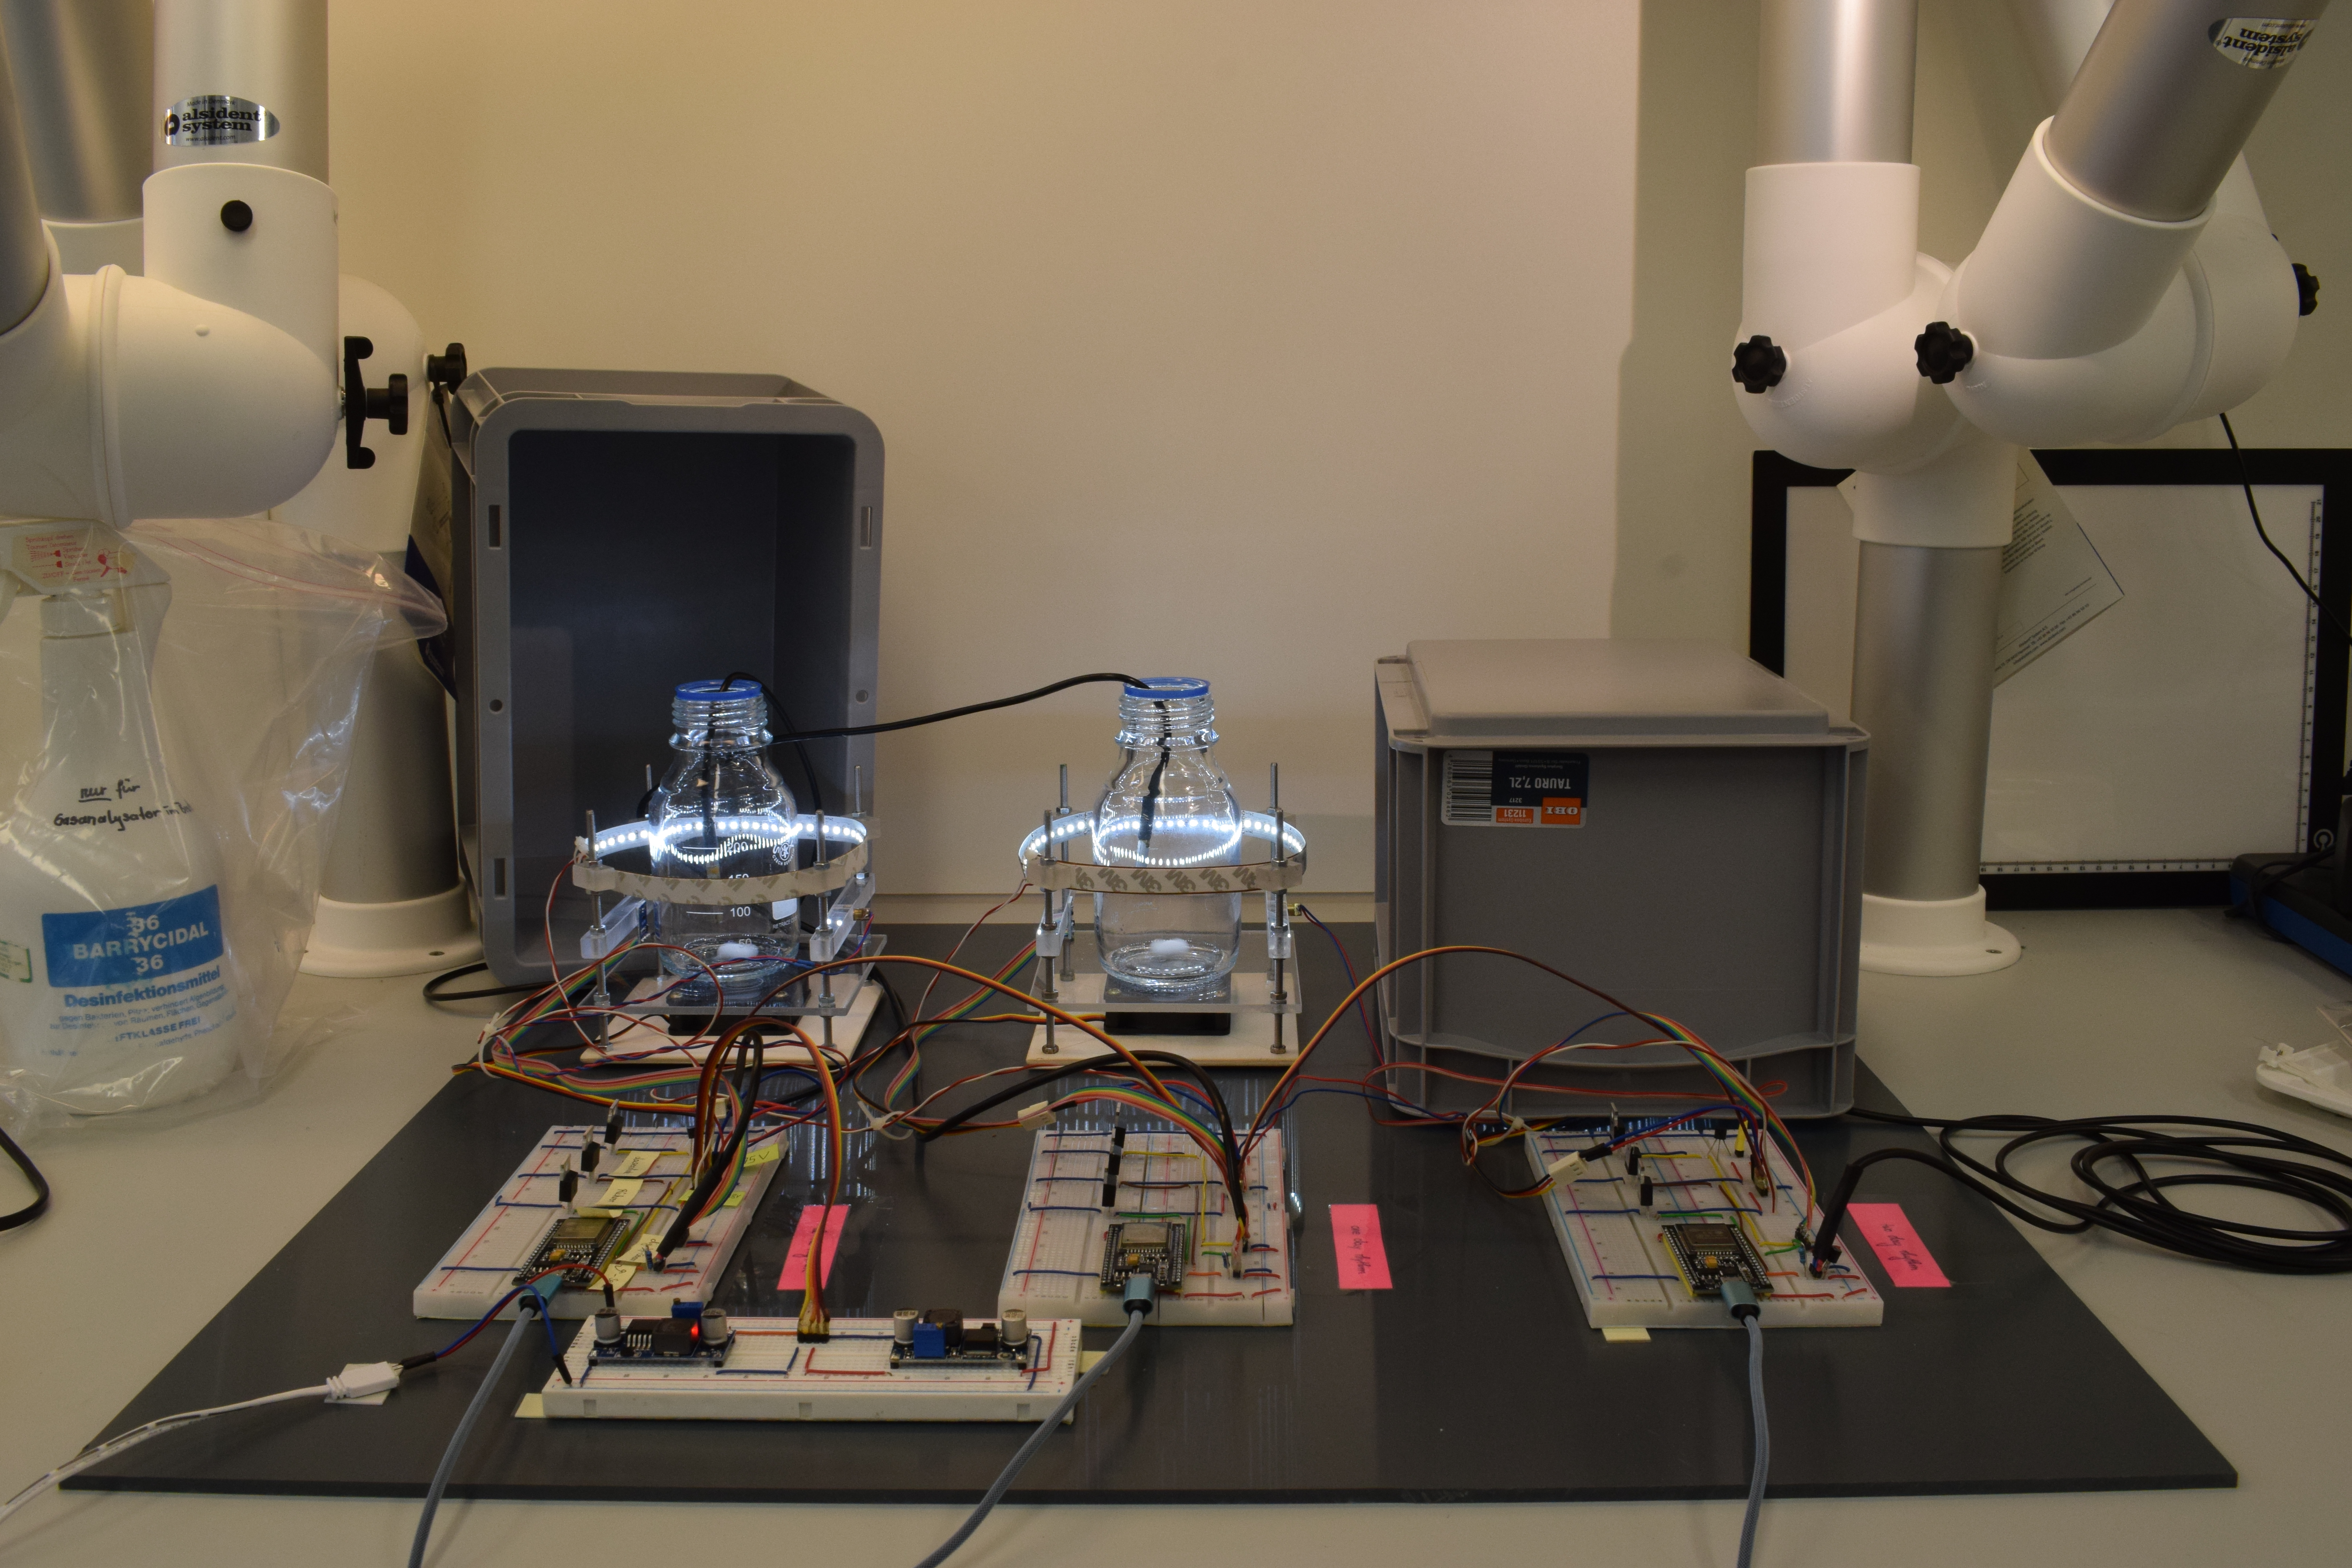
\includegraphics{komplett_mit Licht_mit Kisten.jpg} \#\# Technik

\includegraphics{Controller_Steckbrett.jpg} gegebenenfalls Tabelle mit
genauer Bezeichnung und Grund der Verwendung - damit spart man sich Text
- wird eher gelesen und ist übersichtlicher

\includegraphics{step_up_Modul_Steckbrett.jpg} hier kurz deren Bedeutung
erläutern

\includegraphics{Hauptsteckbrett_Steckplatine_fritzing.png} hier ggf
darauf eingehen, dass ja Massenproduktion erfolgen könnte - verdrahtete
Steckbretter hierfür sinnvoll

\hypertarget{software}{%
\subsection{Software}\label{software}}

RSkript hier bitte einfügen und Kurzbeschriebung, was es tut.

\hypertarget{auswertung-der-daten}{%
\section{Auswertung der Daten}\label{auswertung-der-daten}}

\hypertarget{kalibrierung}{%
\subsection{Kalibrierung}\label{kalibrierung}}

\begin{figure}
\centering
\includegraphics{Kalibrierfunktion.png}
\caption{lineare Kalibrierfunktion}
\end{figure}

\hypertarget{wachstumskurven}{%
\subsection{Wachstumskurven}\label{wachstumskurven}}

\begin{figure}
\centering
\includegraphics{Wachstumskurve_Versuch02_lr01.png}
\caption{Wachstumskurve lr01 (welche hell-dunkel ZEiten?)}
\end{figure}

\includegraphics{Wachstumskurve Vorversuch 3.png} \#\# Wachstumsrate

\begin{figure}
\centering
\includegraphics{Wachstumsrate.png}
\caption{Wachstumsrate}
\end{figure}

\end{document}
